\documentclass{/home/daniel/GitHub/USC-Physics-Degree-Notes/Notes/Presentacion}

\usetheme{Berlin}
\usecolortheme{default}
\RequirePackage{booktabs}
\setbeamersize{text margin left=10pt, text margin right=10pt}
\addbibresource{sample.bib} % si quieres incluir la bibliografía


%----------------------------------------------------------------------------------------
%    TITLE PAGE
%----------------------------------------------------------------------------------------

\title{Práctica de Electronica con ABACUS-Nanohub}
\subtitle{Capacitor MOS}

\author{Daniel Vázquez Lago}

%\institute
%{
%    Department of Computer Science and Information Engineering \\
%    National Taiwan University % Your institution for the title page
%}
\date{\today} % Date, can be changed to a custom date

%----------------------------------------------------------------------------------------
%    PRESENTATION SLIDES
%----------------------------------------------------------------------------------------

\begin{document}

\begin{frame}
    % Print the title page as the first slide
    \titlepage
\end{frame}
\begin{frame}
    % Print the title page as the first slide
    \tableofcontents
\end{frame}

\section{Objetivos}
\begin{frame}{Objetivos}
    Nuestro objetivo es analizar un capacitor MOS. En particular representaremos y daremos los valores caracterísicos para los siguientes casos:
    \begin{itemize}
        \item Diagarama de bandas en equilibrio y en polarización.
        \item Densidad de electrones y huecos en equlibrio y en polarización.
        \item Potencial electrostático y campo elećtrico en equlbirio y con polarizaciones.
        \item Calcular el valor de la función de trabajo del metal para estar en condiciones de banda plana en equilibrio termodinámico. 
    \end{itemize}
    Es muy \textbf{importante} recalcar lo siguiente: la herramienta proporcionada ABACUS Nanohub solo nos permite obtener valores en la parte del semiconductor, por lo que nosotros nos centraremos en esta principalmente.
\end{frame}

%----------------------------------------------------------------------------------------

\section{Parametros}

\begin{frame}{Parámetros del capacitor}
    Los parámetros que introducimos en la simulación: 
    \begin{center} 
        \begin{tabular}{ccccccc} \toprule
            $N_A$ [cm$^{-3}$] & $x_{ox}$ [$\mu$m] & $x_{sc}$  [$\mu$m] & $T$ [K] & $K_{S}$ & $K_S$ & $n_i$  [cm$^{-3}$] \\ \midrule
            $\SI{3.5e+14}{}$ & $\SI{0.1}{}$ & $\SI{5}{}$ & $\SI{3e+2}{}$ & $\SI{3.9}{}$ & $\SI{11.7}{}$ & $\SI{1e+10}{}$ \\ \bottomrule 
        \end{tabular}
    \end{center}
    \begin{center} 
        \begin{tabular}{cccc} \toprule
            $E_g$ [eV] & $m_h^*/m_e$ &$m_n^*/m_e$ & $\chi$  [eV]\\ \midrule
            $\SI{1.12}{}$ & $\SI{0.81}{}$ & $\SI{1.18}{}$ & 4.05  \\ \bottomrule 
        \end{tabular}
    \end{center}
\end{frame}

%---------------------------------------------------------------------------------------

\section{Introducción teórica}
\begin{frame}{Aproximación del MOS ideal.}
    Para los cálculos teóricos vamos a realizar una serie de suposiciones:

    \begin{itemize}
        \item El potencial en el metal es constante.
        \item El óxido es perfecto: no hay corrientes a través de esta.
        \item No hay centros de carga en el óxido ni en las interfaces. 
        \item El semiconductor está uniformemente dopado. 
        \item El semiconductor es suficientemente ancho como para que en la zona del contacto óhmico las bandas sean planas.
        \item Las funciones de trabajo del semiconductor y del metal son iguales.
    \end{itemize}
\end{frame}

\begin{frame}{Definiciones básicas}
    Aquí definimos puntos clave y básicos en las ecuaciones: 
    \begin{itemize}
        \item Potencial de puerta $V_G$. Es la diferencia de potencial entre el nivel del metal y el nivel de Fermi en el semiconductor. 
        
        \begin{equation*}
            V_G = \frac{1}{q} (E_F(semiconductor) - E_F(metal))
        \end{equation*}

        \item Potencial de sustrato $\phi_b$. Es la diferencia entre el nivel intrínseco $E_i$ y el nivel de Fermi del semicondtor en el sustrato dividido por $q$:
        \begin{equation*}
            \phi_b = \frac{1}{q} (E_i (sustrato) - E_F)
        \end{equation*}
        \item Potencial de interfaz $\phi_s$. Es la diferencia entre el nivel intrínseco en el sustrado y la interfaz dividido por $q$. 
        \begin{equation*}
            \phi_s = \frac{1}{q} (E_i (sustrato) - E_i(interfaz))
        \end{equation*}
    \end{itemize}
\end{frame}

\begin{frame}{Corrección de $V_G$}
    Como hemos dicho $V_G$ es la diferencia entre un nivel de fermi y otro. Si las dos funciones de trabajo son iguales tal y como heoms indicado, y la polarización qeu aplicamos es de 0 V, entonces $V_G=0$. Sin embargo en el capacitor MOS de ABACUS Nanohub esto no es cierto, cuando la polarización aplicada es cero tenemos que $V_G \neq 0$. \\
    
    Esto es porque las \textit{funciones de trabajo no son iguales}, de tal forma que 
    \begin{equation*}
        V_G'  = V_{FB} + V_{polarizacion} 
    \end{equation*}
    siendo $V_{FB}$ la \textbf{tensión de banda plana}. Como veremos $V_{FB}$ es elevada, por lo que hará que, aunque menor que la tensión umbral. Así pues lo que haremos será calcular primero $V_{FB}$ a partir de la simulación y usaremos $V_G'$ para los cálculos teóricos en vez de $V_G=V_{ideal}  = V_{polarizacion}$.
\end{frame}

\begin{frame}{Banda plana, acumulación, vaciamiento e inversa.}
    En función del valor de $V_G$ tendremos un valor de $\phi_s$.  Para un portador tipo $N$, en función del valor de $\phi_s$ podemos distinguir 
    \begin{itemize}
        \item \textbf{Acmulación $\phi_s<0$}. Ocurre cuando $V_G'<0$.
        \item \textbf{Equilibrio $\phi_S=0$}. Ocurre solo cuando $V_G'=0$.
        \item \textbf{Vaciamiento $0< \phi_S <2\phi_b$}.  Ocurre cuando $0<V_G'<V_T$.
        \item \textbf{Inversión $2\phi_b<\phi_S$}. Ocurre cuando $V_G'>V_T$.
    \end{itemize}
    Definimos $V_T$ como el potencial umbral, y lo podemos obtener como: 

    \begin{equation*}
        V_T = 2 \phi_b + \frac{K_S}{k_{ox}} x_{ox} \sqrt{\frac{4qN_D}{K_S\varepsilon_0} \phi_b} = 0.78 \ \unit{V}
    \end{equation*}
    Mientras que $\phi_b$, al estar definido en el sustrato cuando $x\rightarrow\infty$ tenemos que es un parámetro que depende solo del material, dopado (tipo $N$) y temperatura: 

    \begin{equation*}
        \phi_b = \frac{kT}{q} \log \left( \frac{N_A}{n_i}\right) = 0.27 \ \unit{V}
    \end{equation*}    

\end{frame}


\begin{frame}{Densidad de huecos y electrones en la interfaz}
    Y los valores de la densidad de huecos y electrones dependerán de si estamos en la región de acumulación, vaciamiento o inversión: 
    \begin{itemize}
        \item \textbf{Acmulación}.
        \begin{equation*}
            p_p =  n_i e^{(E_F-E_i)/k T}  \qquad n_p = \frac{n_i^2}{p_p}
        \end{equation*}
        \item \textbf{Vaciamiento}. Válido cuando vaciamiento delta. 
        \begin{equation*}
            p_p \approx n_i  \qquad n_p \approx n_i
        \end{equation*}
        \item \textbf{Inversión}. 
        \begin{equation*}
            n_p =  n_i e^{-(E_F-E_i)/k T}  \qquad p_p = \frac{n_i^2}{n_p}
        \end{equation*}
    \end{itemize}
    Recordamos que la densidad de carga es: 
    \begin{equation*}
        \rho = q (p_p - n_p - N_A)
    \end{equation*}
\end{frame}

\begin{frame}{Densidad de huecos y electrones en el sustrato}
    En el sustrato cuando $x=5\mu m$ deberíamos encontrarnos el caso del semiconductor extrínseco con los dopantes ionizados típico, tal que: 
    \begin{equation}
        p_p \approx N_A \qquad n_p = \frac{n_i^2}{N_A}
    \end{equation}
\end{frame}

\begin{frame}{Aproximación de vaciamiento delta}
    Además de las aproximaciones mencionadas anteriormente tenemos que suponer la aproximación de vaciamiento delta. La aproximación de vaciamiento delta nos permite obtener los valores de $\phi_S$, $\Ecal(x)$, $V(x)$ y $\rho(x)$ a lo largo del semiconductor. 

    \hspace*{1em}

    Esta aproximación solo es valida en la región de vaciamiento $0<V_G'<0.78$ V, y asume que hace es suponer que en la región $0\leq x \leq W$ del semiconductor es $\rho(x) \approx -qN_A$. Como veremos, con ninguno de los potenciales de polarización será valida la aproximación de vaciamiento delta, y por tanto todas los resultados teóricos diferiran mucho de la simulación. 
\end{frame}
\begin{frame}{Valor de $\phi_s$ y bandas}
    El valor $\phi_s$ en el semiconductor dependen en última instancia del potencial $V_G$ que le demos, que será nuestro parámetro de entrada. Así pues, dado un $V_G$, tenemos que:

    \begin{equation*}
        \phi_s = \text{sign}(V_G) \left( \frac{-\alpha+ \sqrt{\alpha^2 + 4|V_G|}}{2} \right)^2 \qquad \alpha^2 =  \left(\frac{K_S}{K_{ox}} x_0 \sqrt{\frac{2qN_A}{K_S\varepsilon_0}}  \right)^2=  0.097 \ \unit{V}
    \end{equation*}
    Y por otro lado las bandas ($E_F=0$) donde $E_i=\frac{kT}{q}\log \left(\frac{N_A}{n_i}\right)$:

    \begin{equation*}
        E_c (sustrato) = \frac{E_g}{2} + \frac{3}{4} kT \log\left(\frac{m_p^*}{m_n^*}\right) + E_i \quad 
        E_v (sustrato) = - \frac{E_g}{2} + \frac{3}{4} kT \log\left(\frac{m_p^*}{m_n^*}\right) + E_i
    \end{equation*} 
    y en la interfaz
    \begin{equation*}
        E_c (interfaz) = E_c (sustrato) + \phi_s  \qquad
        E_v (interfaz) = E_v (sustrato) + \phi_s
    \end{equation*}

\end{frame}
\begin{frame}{Campo eléctrico y en la interfaz}
    El valor del campo elećtrico en la interfaz: 
    \begin{equation*}
        \Ecal (interfaz) = \frac{qN_D}{K_S\varepsilon_0} W \qquad W = \sqrt{\frac{2K_S\varepsilon_0}{qN_A} \phi_s}
    \end{equation*}
    Que lo indicaremos en las tablas como $\Ecal_{sc}$. Además tendremos 

    \begin{equation}
        \Ecal_{ox} = \frac{K_S}{K_{ox}} \Ecal_{sc}
    \end{equation}
    en virtud de las condiciones de frontero óxido-semiconductor.

\end{frame}
%%%%%%%%%%%%%%%%%%%%%%%%%%%%%%%%%%%%%%%%%%%%%%%%%%%%%%%%%%%%%%%%%%%%%%
%%%%%%%%%%%%%%%%%%%%%%%%%%%%%%%%%%%%%%%%%%%%%%%%%%%%%%%%%%%%%%%%%%%%%%
%%%%%%%%%%%%%%%%%%%%%%%%%%%%%%%%%%%%%%%%%%%%%%%%%%%%%%%%%%%%%%%%%%%%%%
%%%%%%%%%%%%%%%%%%%%%%%%%%%%%%%%%%%%%%%%%%%%%%%%%%%%%%%%%%%%%%%%%%%%%%

\section{Tensión de banda plana}

\begin{frame}{Tensión de banda plana}
    Para el calculo de la tensión de banda plana vamos a calcular $V_G$, a partir del $\phi_S$ cuando $V_{polarizacion}=0$, ya que por definición esto implicaría que:

    \begin{equation}
        V_G = V_{FB}
    \end{equation}
    Como veremos $\phi_S=0.58$ V, tal que $\phi_S \approx 2 \phi_b$, estando en el rango de aplicación de la aproximación de vaciamiento, de lo que obtenemos: 

    \begin{equation}
        V_{FB}= 0.82 \ \unit{V}
    \end{equation}
    Así pues, a partir de ahora:

    \begin{equation}
        V_G' = V_G (ideal) - V_{FB}
    \end{equation}

\end{frame}

%%%%%%%%%%%%%%%%%%%%%%%%%%%%%%%%%%%%%%%%%%%%%%%%%%%%%%%%%%%%%%%%%%%%%%
%%%%%%%%%%%%%%%%%%%%%%%%%%%%%%%%%%%%%%%%%%%%%%%%%%%%%%%%%%%%%%%%%%%%%%
%%%%%%%%%%%%%%%%%%%%%%%%%%%%%%%%%%%%%%%%%%%%%%%%%%%%%%%%%%%%%%%%%%%%%%
%%%%%%%%%%%%%%%%%%%%%%%%%%%%%%%%%%%%%%%%%%%%%%%%%%%%%%%%%%%%%%%%%%%%%%

\section{$V_{pol}=0$} 

\begin{frame}{Potencial electrostático y anchura}
    \begin{minipage}{0.4\linewidth}
        Estamos en inversión, ya que $V_G'=0.82>V_T=0.78$.
        
        \vspace*{1em}
        
        \begin{center}
            \small
            \begin{tabular}{ccc}
                \toprule
                & $\phi_S$ [V] & $W$ [$\mu$m]   \\ \midrule
                Teoria & $\SI{5.8e-01}{}$ & $\SI{1.46}{}$ \\
                Sim.   & $\SI{5.8e-01}{}$ & $\SI{1.88}{}$  \\
                \bottomrule
            \end{tabular}
        \end{center}
    \end{minipage}
    \hfill
    \begin{minipage}{0.55\linewidth} \centering
        Potencial electrósticatico en función de x:

        \vspace*{1em}
        
        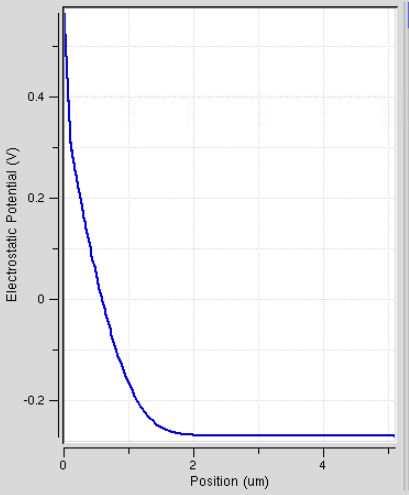
\includegraphics[width=0.7\linewidth]{../Imagenes/0-Potencial.png}
    \end{minipage}
\end{frame}


\begin{frame}{Bandas de energía}
    \begin{minipage}{0.4\linewidth}
        \begin{center}
            \small
            En la interfaz ($E_F=0$ eV)
            \vspace*{1em}

            \begin{tabular}{ccc}
                \toprule
                & $E_c $ [eV] & $E_v $ [eV]  \\ \midrule
                Teoria &  $\SI{8.23e-01}{}$& $\SI{-2.97e-01}{}$\\
                Sim. &  $\SI{8.63e-01}{}$& $\SI{-2.83e-01}{}$  \\
                \bottomrule
            \end{tabular}

            \vspace*{2em}

            En el sustrato ($E_F=0$ eV) 

            \vspace*{1em}

            \begin{tabular}{ccc}
                \toprule
                & $E_c $ [eV] & $E_v $ [eV]  \\ \midrule
                Teoria & $\SI{2.43e-01}{}$ & $\SI{-8.77e-01}{}$ \\
                Sim. & $\SI{2.57e-01}{}$ & $\SI{-8.63e-01}{}$ \\
                \bottomrule
            \end{tabular}
        \end{center}
    \end{minipage}
    \hfill
    \begin{minipage}{0.55\linewidth}\centering

        Bandas en el semiconductor. \textcolor{blue}{Azul}: $E_c$. \textcolor{Green}{Verde}: $E_v$.  

        \vspace*{1em}
        
        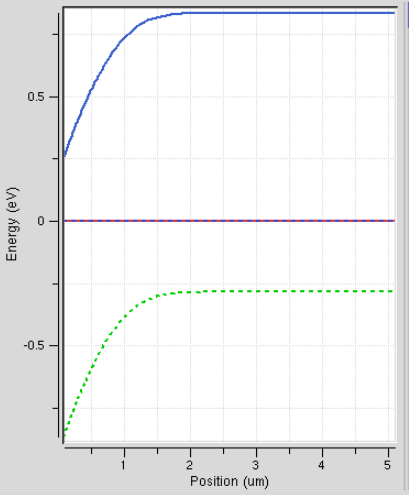
\includegraphics[width=0.7\linewidth]{../Imagenes/0-Band.png}
    \end{minipage}
\end{frame}


\begin{frame}{Densidad de portadores}
    \begin{minipage}{0.4\linewidth}
        \begin{center}
            \small
            En la interfaz: 
            \vspace*{1em}

            \begin{tabular}{ccc}
                \toprule
                & $n_p $ [cm$^{-3}$] & $p_p $ [cm$^{-3}$]  \\ \midrule
                Teoria & $\SI{1.58e+15}{}$& $\SI{6.34e+04}{}$ \\

                Sim. & $\SI{1.57e+15}{}$ & $\SI{6.34e+04}{}$  \\
                \bottomrule
            \end{tabular}

            \vspace*{2em}

            En el sustrato: 

            \vspace*{1em}


            \begin{tabular}{ccc}
                \toprule
                & $n_p $ [cm$^{-3}$] & $p_p $ [cm$^{-3}$]  \\ \midrule
                Teoria & $\SI{2.86e+05}{}$ & $\SI{3.50e+14}{}$ \\
                Sim. & $\SI{2.83e+05}{}$ & $\SI{3.50e+14}{}$ \\
                \bottomrule
            \end{tabular}

        \end{center}
    \end{minipage}
    \hfill
    \begin{minipage}{0.55\linewidth}\centering

        Densidad de carga.

        \vspace*{0.5em}

        \textcolor{blue}{Azul}: $n_p$. \textcolor{red}{Rojo}: $p_p$. \textcolor{Green}{Verde}: $\rho$.  

        \vspace*{1em}

        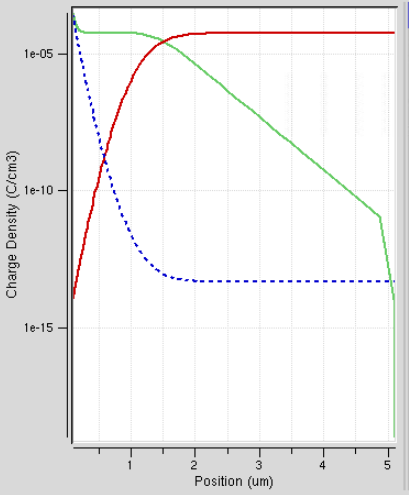
\includegraphics[width=0.65\linewidth]{../Imagenes/0-Charge.png}
    \end{minipage}
\end{frame}

\begin{frame}{Campo eléctrico}
    \begin{minipage}{0.4\linewidth}
        \begin{center}
            \small
            En la interfaz: 
            \vspace*{1em}

            \begin{tabular}{ccc}
                \toprule
                & $\Ecal_{ox} $ [V/cm] & $\Ecal_{sc} $ [V/cm]   \\ \midrule
                Teoria &  $\SI{2.38e+04}{}$ &  $\SI{7.92e+03}{}$ \\
                Sim. &  $\SI{2.57e+04}{}$ &  $\SI{8.49e+03}{}$  \\
                \bottomrule
            \end{tabular}
        \end{center}
    \end{minipage}
    \hfill
    \begin{minipage}{0.55\linewidth} 
        \centering
        Campo eléctrico.
        \vspace*{1em}
        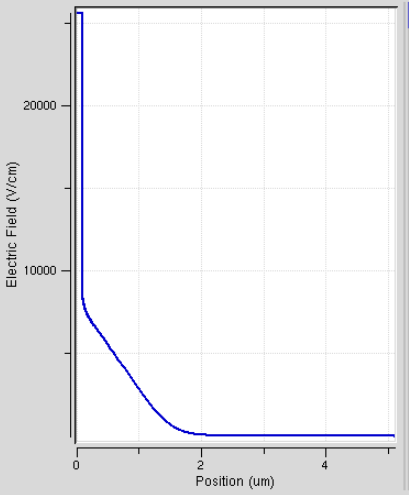
\includegraphics[width=0.7\linewidth]{../Imagenes/0-Field.png}
    \end{minipage}
\end{frame}

%%%%%%%%%%%%%%%%%%%%%%%%%%%%%%%%%%%%%%%%%%%%%%%%%%%%%%%%%%%%%%%%%%%%%%
%%%%%%%%%%%%%%%%%%%%%%%%%%%%%%%%%%%%%%%%%%%%%%%%%%%%%%%%%%%%%%%%%%%%%%
%%%%%%%%%%%%%%%%%%%%%%%%%%%%%%%%%%%%%%%%%%%%%%%%%%%%%%%%%%%%%%%%%%%%%%
%%%%%%%%%%%%%%%%%%%%%%%%%%%%%%%%%%%%%%%%%%%%%%%%%%%%%%%%%%%%%%%%%%%%%%

\section{$V_{pol}=+2$ V} 


\begin{frame}{Potencial electrostático y anchura}
    \begin{minipage}{0.4\linewidth}
        \begin{center}
            \small
            Estamos en inversión, ya que $V_G'=2.82>V_T=0.78$.
            
            \vspace*{1em}

            \begin{tabular}{ccc}
                \toprule
                & $\phi_S$ [V] & $W$ [$\mu$m]   \\ \midrule
                Teoria & $\SI{2.34e+00}{}$ & $\SI{2.94}{}$ \\
                Sim.   & $\SI{7.35e-01}{}$ & $\SI{1.97}{}$  \\
                \bottomrule
            \end{tabular}
        \end{center}
    \end{minipage}
    \hfill
    \begin{minipage}{0.55\linewidth} \centering
        Potencial electrósticatico en función de x:

        \vspace*{1em}
        
        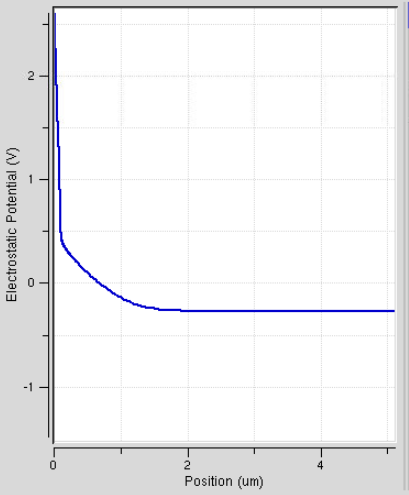
\includegraphics[width=0.7\linewidth]{../Imagenes/1-Potencial.png}
    \end{minipage}
\end{frame}


\begin{frame}{Bandas de energía}
    \begin{minipage}{0.4\linewidth}
        \begin{center}
            \small
            En la interfaz ($E_F=0$ eV)
            \vspace*{1em}

            \begin{tabular}{ccc}
                \toprule
                & $E_c $ [eV] & $E_v $ [eV]  \\ \midrule
                Teoria &  $\SI{-1.52e-00}{}$& $\SI{-2.64e+00}{}$\\
                Sim. &  $\SI{1.02e-01}{}$& $\SI{-1.02e+00}{}$  \\
                \bottomrule
            \end{tabular}

            \vspace*{2em}

            En el sustrato ($E_F=0$ eV) 

            \vspace*{1em}

            \begin{tabular}{ccc}
                \toprule
                & $E_c $ [eV] & $E_v $ [eV]  \\ \midrule
                Teoria & $\SI{2.43e-01}{}$ & $\SI{-8.77e-01}{}$ \\
                Sim. & $\SI{2.57e-01}{}$ & $\SI{-8.63e-01}{}$ \\
                \bottomrule
            \end{tabular}
        \end{center}
    \end{minipage}
    \hfill
    \begin{minipage}{0.55\linewidth}\centering

        Bandas en el semiconductor. \textcolor{blue}{Azul}: $E_c$. \textcolor{Green}{Verde}: $E_v$.  

        \vspace*{1em}
        
        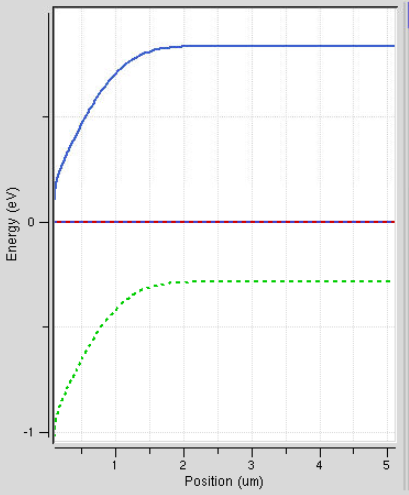
\includegraphics[width=0.7\linewidth]{../Imagenes/1-Band.png}
    \end{minipage}
\end{frame}


\begin{frame}{Densidad de portadores}
    \begin{minipage}{0.4\linewidth}
        \begin{center}
            \small
            En la interfaz: 
            \vspace*{1em}

            \begin{tabular}{ccc}
                \toprule
                & $n_p $ [cm$^{-3}$] & $p_p $ [cm$^{-3}$]  \\ \midrule
                Teoria &$\SI{5.86e+44}{}$& $\SI{1.71e-25}{}$\\

                Sim. & $\SI{1.57e+15}{}$ & $\SI{6.34e+05}{}$  \\
                \bottomrule
            \end{tabular}

            \vspace*{2em}

            En el sustrato: 

            \vspace*{1em}


            \begin{tabular}{ccc}
                \toprule
                & $n_p $ [cm$^{-3}$] & $p_p $ [cm$^{-3}$]  \\ \midrule
                Teoria & $\SI{2.86e+05}{}$ & $\SI{3.50e+14}{}$ \\
                Sim. & $\SI{2.83e+05}{}$ & $\SI{3.50e+14}{}$ \\
                \bottomrule
            \end{tabular}

        \end{center}
    \end{minipage}
    \hfill
    \begin{minipage}{0.55\linewidth}\centering

        Densidad de carga.

        \vspace*{0.5em}

        \textcolor{blue}{Azul}: $n_p$. \textcolor{red}{Rojo}: $p_p$. \textcolor{Green}{Verde}: $\rho$.  

        \vspace*{1em}

        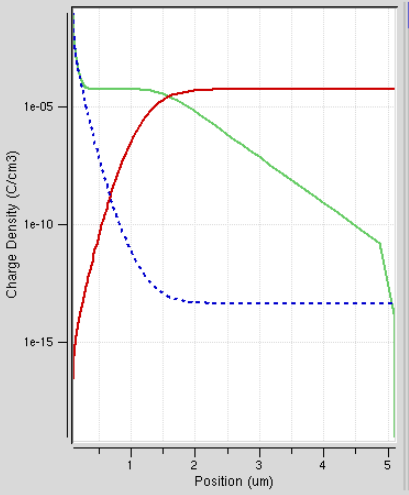
\includegraphics[width=0.65\linewidth]{../Imagenes/1-Charge.png}
    \end{minipage}
\end{frame}

\begin{frame}{Campo eléctrico}
    \begin{minipage}{0.4\linewidth}
        \begin{center}
            \small
            En la interfaz: 
            \vspace*{1em}

            \begin{tabular}{ccc}
                \toprule
                & $\Ecal_{ox} $ [V/cm] & $\Ecal_{sc} $ [V/cm]   \\ \midrule
                Teoria &  $\SI{4.77e+04}{}$ &  $\SI{1.59e+04}{}$ \\
                Sim. &  $\SI{2.14e+05}{}$ &  $\SI{7.00e+04}{}$  \\
                \bottomrule
            \end{tabular}
        \end{center}
    \end{minipage}
    \hfill
    \begin{minipage}{0.55\linewidth} 
        \centering
        Campo eléctrico.
        \vspace*{1em}
        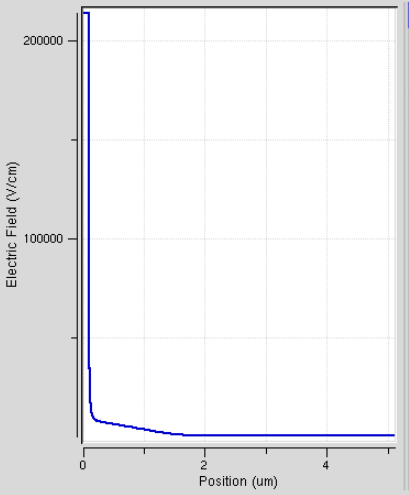
\includegraphics[width=0.7\linewidth]{../Imagenes/1-Field.png}
    \end{minipage}
\end{frame}

%%%%%%%%%%%%%%%%%%%%%%%%%%%%%%%%%%%%%%%%%%%%%%%%%%%%%%%%%%%%%%%%%%%%%%
%%%%%%%%%%%%%%%%%%%%%%%%%%%%%%%%%%%%%%%%%%%%%%%%%%%%%%%%%%%%%%%%%%%%%%
%%%%%%%%%%%%%%%%%%%%%%%%%%%%%%%%%%%%%%%%%%%%%%%%%%%%%%%%%%%%%%%%%%%%%%
%%%%%%%%%%%%%%%%%%%%%%%%%%%%%%%%%%%%%%%%%%%%%%%%%%%%%%%%%%%%%%%%%%%%%%

\section{$V_{pol}=-2$ V} 


\begin{frame}{Potencial electrostático y anchura}
    \begin{minipage}{0.4\linewidth}
        Estamos en acumulación, ya que $V_G'=-1.18<0.0$.
        
        \vspace*{1em}

        \begin{center}
            \small
            \begin{tabular}{ccc}
                \toprule
                & $\phi_S$ [V] & $W$ [$\mu$m]   \\ \midrule
                Teoria & $\SI{-8.88e-01}{}$ & $\SI{1.81}{}$ \\
                Sim.   & $\SI{-1.57e-01}{}$ & $\SI{0.99}{}$  \\
                \bottomrule
            \end{tabular}
        \end{center}
    \end{minipage}
    \hfill
    \begin{minipage}{0.55\linewidth} \centering
        Potencial electrósticatico en función de x:

        \vspace*{1em}
        
        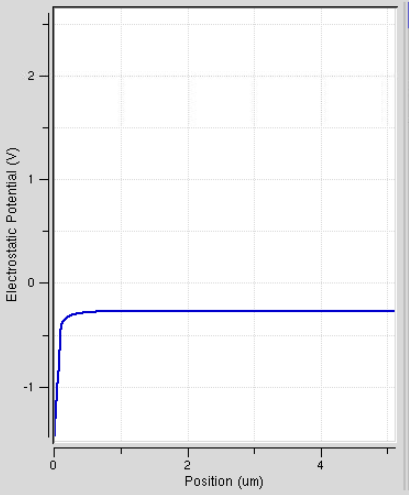
\includegraphics[width=0.7\linewidth]{../Imagenes/2-Potencial.png}
    \end{minipage}
\end{frame}


\begin{frame}{Bandas de energía}
    \begin{minipage}{0.4\linewidth}
        \begin{center}
            \small
            En la interfaz ($E_F=0$ eV)
            \vspace*{1em}
            \begin{tabular}{ccc}
                \toprule
                & $E_c $ [eV] & $E_v $ [eV]  \\ \midrule
                Teoria &  $\SI{1.71e+00}{}$& $\SI{5.91e-01}{}$\\
                Sim. &  $\SI{9.94e-01}{}$& $\SI{-1.236e-01}{}$  \\
                \bottomrule
            \end{tabular}

            \vspace*{2em}

            En el sustrato ($E_F=0$ eV) 

            \vspace*{1em}

            \begin{tabular}{ccc}
                \toprule
                & $E_c $ [eV] & $E_v $ [eV]  \\ \midrule
                Teoria & $\SI{2.43e-01}{}$ & $\SI{-8.77e-01}{}$ \\
                Sim. & $\SI{2.57e-01}{}$ & $\SI{-8.63e-01}{}$ \\
                \bottomrule
            \end{tabular}
        \end{center}
    \end{minipage}
    \hfill
    \begin{minipage}{0.55\linewidth}\centering

        Bandas en el semiconductor. \textcolor{blue}{Azul}: $E_c$. \textcolor{Green}{Verde}: $E_v$.  

        \vspace*{1em}
        
        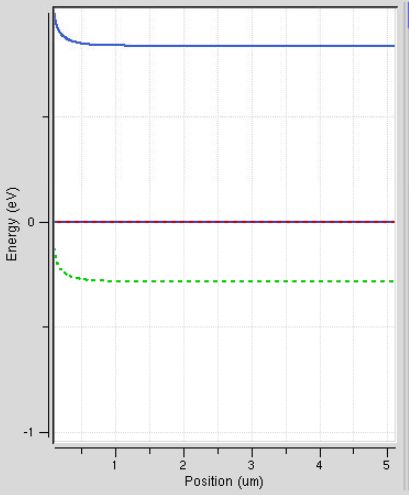
\includegraphics[width=0.7\linewidth]{../Imagenes/2-Band.png}
    \end{minipage}
\end{frame}


\begin{frame}{Densidad de portadores}
    \begin{minipage}{0.4\linewidth}
        \begin{center}
            \small
            En la interfaz: 
            \vspace*{1em}
            \begin{tabular}{ccc}
                \toprule
                & $n_p $ [cm$^{-3}$] & $p_p $ [cm$^{-3}$]  \\ \midrule
                Teoria &$\SI{2.92e+29}{}$& $\SI{1.71e-25}{}$ \\
                Sim. & $\SI{1.53e+17}{}$ & $\SI{6.47e+02}{}$ \\
                \bottomrule
            \end{tabular}

            \vspace*{2em}

            En el sustrato: 

            \vspace*{1em}


            \begin{tabular}{ccc}
                \toprule
                & $n_p $ [cm$^{-3}$] & $p_p $ [cm$^{-3}$]  \\ \midrule
                Teoria & $\SI{2.86e+05}{}$ & $\SI{3.50e+14}{}$ \\
                Sim. & $\SI{2.83e+05}{}$ & $\SI{3.50e+14}{}$ \\
                \bottomrule
            \end{tabular}

        \end{center}
    \end{minipage}
    \hfill
    \begin{minipage}{0.55\linewidth}\centering

        Densidad de carga.

        \vspace*{0.5em}

        \textcolor{blue}{Azul}: $n_p$. \textcolor{red}{Rojo}: $p_p$. \textcolor{Green}{Verde}: $\rho$.  

        \vspace*{1em}

        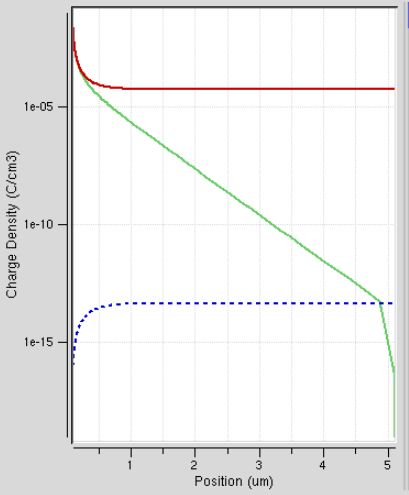
\includegraphics[width=0.65\linewidth]{../Imagenes/2-Charge.png}
    \end{minipage}
\end{frame}

\begin{frame}{Campo eléctrico}
    \begin{minipage}{0.4\linewidth}
        \begin{center}
            \small
            En la interfaz: 
            \vspace*{1em}

            \begin{tabular}{ccc}
                \toprule
                & $\Ecal_{ox} $ [V/cm] & $\Ecal_{sc} $ [V/cm]   \\ \midrule
                Teoria & $ \SI{2.94e+04}{}$ & $\SI{9.81e+03}{}$ \\
                Sim. &  $\SI{1.04e+05}{}$ &  $\SI{3.44e+04}{}$  \\
                \bottomrule
            \end{tabular}
        \end{center}
    \end{minipage}
    \hfill
    \begin{minipage}{0.55\linewidth} 
        \centering
        Campo eléctrico.
        \vspace*{1em}
        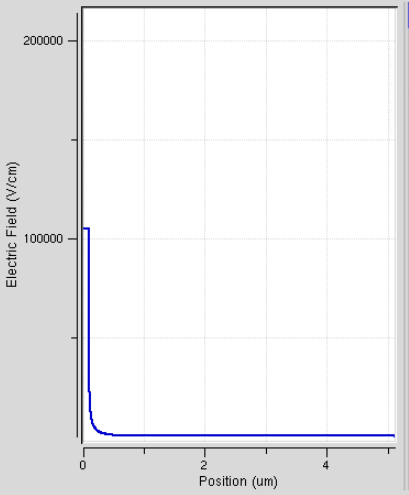
\includegraphics[width=0.7\linewidth]{../Imagenes/2-Field.png}
    \end{minipage}
\end{frame}

%%%%%%%%%%%%%%%%%%%%%%%%%%%%%%%%%%%%%%%%%%%%%%%%%%%%%%%%%%%%%%%%%%%%%%
%%%%%%%%%%%%%%%%%%%%%%%%%%%%%%%%%%%%%%%%%%%%%%%%%%%%%%%%%%%%%%%%%%%%%%
%%%%%%%%%%%%%%%%%%%%%%%%%%%%%%%%%%%%%%%%%%%%%%%%%%%%%%%%%%%%%%%%%%%%%%
%%%%%%%%%%%%%%%%%%%%%%%%%%%%%%%%%%%%%%%%%%%%%%%%%%%%%%%%%%%%%%%%%%%%%%

\section{Función de trabajo}

\begin{frame}{Función de trabajo}
    La función de trabajo la calculamos como: 
    \begin{equation}
        \phi_m = q\chi  + (E_C-E_F)_{sustrato} - q V_{TB} = 4.05 + 0.863 - 0.82 = 4.078 \ \unit{eV}
    \end{equation}
    que correspondería a la función de trabajo del aluminio o indio (que estarían en un intervalo de 4.1 a 4.5 eV). 
\end{frame}

\section{Conclusiones}

\begin{frame}{Conclusiones}
    \begin{minipage}{0.9\linewidth}
    Las conclusiones finales son: 

    \begin{itemize}
        \item Los voltajes dados son demasiado grandes: no tenemos ecuaciones analíticas para inversión y acumulación. 
        \item El comportamiento de la simulación es el esperado. 
    \end{itemize}
    \end{minipage}
\end{frame}

\begin{frame}
    \begin{center}
    \Huge{\textbf{FIN}}
    \end{center}
\end{frame}






\end{document}
